% Options for packages loaded elsewhere
\PassOptionsToPackage{unicode}{hyperref}
\PassOptionsToPackage{hyphens}{url}
%
\documentclass[
]{article}
\usepackage{amsmath,amssymb}
\usepackage{lmodern}
\usepackage{iftex}
\ifPDFTeX
  \usepackage[T1]{fontenc}
  \usepackage[utf8]{inputenc}
  \usepackage{textcomp} % provide euro and other symbols
\else % if luatex or xetex
  \usepackage{unicode-math}
  \defaultfontfeatures{Scale=MatchLowercase}
  \defaultfontfeatures[\rmfamily]{Ligatures=TeX,Scale=1}
\fi
% Use upquote if available, for straight quotes in verbatim environments
\IfFileExists{upquote.sty}{\usepackage{upquote}}{}
\IfFileExists{microtype.sty}{% use microtype if available
  \usepackage[]{microtype}
  \UseMicrotypeSet[protrusion]{basicmath} % disable protrusion for tt fonts
}{}
\makeatletter
\@ifundefined{KOMAClassName}{% if non-KOMA class
  \IfFileExists{parskip.sty}{%
    \usepackage{parskip}
  }{% else
    \setlength{\parindent}{0pt}
    \setlength{\parskip}{6pt plus 2pt minus 1pt}}
}{% if KOMA class
  \KOMAoptions{parskip=half}}
\makeatother
\usepackage{xcolor}
\IfFileExists{xurl.sty}{\usepackage{xurl}}{} % add URL line breaks if available
\IfFileExists{bookmark.sty}{\usepackage{bookmark}}{\usepackage{hyperref}}
\hypersetup{
  pdftitle={Regression Analysis - STAT 482 - Probem Set 9},
  pdfauthor={Alex Towell (atowell@siue.edu)},
  hidelinks,
  pdfcreator={LaTeX via pandoc}}
\urlstyle{same} % disable monospaced font for URLs
\usepackage[margin=1in]{geometry}
\usepackage{color}
\usepackage{fancyvrb}
\newcommand{\VerbBar}{|}
\newcommand{\VERB}{\Verb[commandchars=\\\{\}]}
\DefineVerbatimEnvironment{Highlighting}{Verbatim}{commandchars=\\\{\}}
% Add ',fontsize=\small' for more characters per line
\usepackage{framed}
\definecolor{shadecolor}{RGB}{248,248,248}
\newenvironment{Shaded}{\begin{snugshade}}{\end{snugshade}}
\newcommand{\AlertTok}[1]{\textcolor[rgb]{0.94,0.16,0.16}{#1}}
\newcommand{\AnnotationTok}[1]{\textcolor[rgb]{0.56,0.35,0.01}{\textbf{\textit{#1}}}}
\newcommand{\AttributeTok}[1]{\textcolor[rgb]{0.77,0.63,0.00}{#1}}
\newcommand{\BaseNTok}[1]{\textcolor[rgb]{0.00,0.00,0.81}{#1}}
\newcommand{\BuiltInTok}[1]{#1}
\newcommand{\CharTok}[1]{\textcolor[rgb]{0.31,0.60,0.02}{#1}}
\newcommand{\CommentTok}[1]{\textcolor[rgb]{0.56,0.35,0.01}{\textit{#1}}}
\newcommand{\CommentVarTok}[1]{\textcolor[rgb]{0.56,0.35,0.01}{\textbf{\textit{#1}}}}
\newcommand{\ConstantTok}[1]{\textcolor[rgb]{0.00,0.00,0.00}{#1}}
\newcommand{\ControlFlowTok}[1]{\textcolor[rgb]{0.13,0.29,0.53}{\textbf{#1}}}
\newcommand{\DataTypeTok}[1]{\textcolor[rgb]{0.13,0.29,0.53}{#1}}
\newcommand{\DecValTok}[1]{\textcolor[rgb]{0.00,0.00,0.81}{#1}}
\newcommand{\DocumentationTok}[1]{\textcolor[rgb]{0.56,0.35,0.01}{\textbf{\textit{#1}}}}
\newcommand{\ErrorTok}[1]{\textcolor[rgb]{0.64,0.00,0.00}{\textbf{#1}}}
\newcommand{\ExtensionTok}[1]{#1}
\newcommand{\FloatTok}[1]{\textcolor[rgb]{0.00,0.00,0.81}{#1}}
\newcommand{\FunctionTok}[1]{\textcolor[rgb]{0.00,0.00,0.00}{#1}}
\newcommand{\ImportTok}[1]{#1}
\newcommand{\InformationTok}[1]{\textcolor[rgb]{0.56,0.35,0.01}{\textbf{\textit{#1}}}}
\newcommand{\KeywordTok}[1]{\textcolor[rgb]{0.13,0.29,0.53}{\textbf{#1}}}
\newcommand{\NormalTok}[1]{#1}
\newcommand{\OperatorTok}[1]{\textcolor[rgb]{0.81,0.36,0.00}{\textbf{#1}}}
\newcommand{\OtherTok}[1]{\textcolor[rgb]{0.56,0.35,0.01}{#1}}
\newcommand{\PreprocessorTok}[1]{\textcolor[rgb]{0.56,0.35,0.01}{\textit{#1}}}
\newcommand{\RegionMarkerTok}[1]{#1}
\newcommand{\SpecialCharTok}[1]{\textcolor[rgb]{0.00,0.00,0.00}{#1}}
\newcommand{\SpecialStringTok}[1]{\textcolor[rgb]{0.31,0.60,0.02}{#1}}
\newcommand{\StringTok}[1]{\textcolor[rgb]{0.31,0.60,0.02}{#1}}
\newcommand{\VariableTok}[1]{\textcolor[rgb]{0.00,0.00,0.00}{#1}}
\newcommand{\VerbatimStringTok}[1]{\textcolor[rgb]{0.31,0.60,0.02}{#1}}
\newcommand{\WarningTok}[1]{\textcolor[rgb]{0.56,0.35,0.01}{\textbf{\textit{#1}}}}
\usepackage{longtable,booktabs,array}
\usepackage{calc} % for calculating minipage widths
% Correct order of tables after \paragraph or \subparagraph
\usepackage{etoolbox}
\makeatletter
\patchcmd\longtable{\par}{\if@noskipsec\mbox{}\fi\par}{}{}
\makeatother
% Allow footnotes in longtable head/foot
\IfFileExists{footnotehyper.sty}{\usepackage{footnotehyper}}{\usepackage{footnote}}
\makesavenoteenv{longtable}
\usepackage{graphicx}
\makeatletter
\def\maxwidth{\ifdim\Gin@nat@width>\linewidth\linewidth\else\Gin@nat@width\fi}
\def\maxheight{\ifdim\Gin@nat@height>\textheight\textheight\else\Gin@nat@height\fi}
\makeatother
% Scale images if necessary, so that they will not overflow the page
% margins by default, and it is still possible to overwrite the defaults
% using explicit options in \includegraphics[width, height, ...]{}
\setkeys{Gin}{width=\maxwidth,height=\maxheight,keepaspectratio}
% Set default figure placement to htbp
\makeatletter
\def\fps@figure{htbp}
\makeatother
\setlength{\emergencystretch}{3em} % prevent overfull lines
\providecommand{\tightlist}{%
  \setlength{\itemsep}{0pt}\setlength{\parskip}{0pt}}
\setcounter{secnumdepth}{-\maxdimen} % remove section numbering
\usepackage{amsmath}
\usepackage{mathtools}
\usepackage{amsthm}
\usepackage{multirow}
\usepackage{booktabs}
\usepackage{minted}
\usepackage{color}
\usepackage{xcolor}
\usepackage{tcolorbox}
\usepackage{enumerate}
\ifLuaTeX
  \usepackage{selnolig}  % disable illegal ligatures
\fi

\title{Regression Analysis - STAT 482 - Probem Set 9}
\author{Alex Towell
(\href{mailto:atowell@siue.edu}{\nolinkurl{atowell@siue.edu}})}
\date{}

\begin{document}
\maketitle

\newcommand{\sos}[1]{\mathrm{SS_{#1}}}
\newcommand{\ms}[1]{\mathrm{MS_{#1}}}
\newcommand{\sd}{\operatorname{sd}}
\newcommand{\var}{\operatorname{var}}
\newcommand{\expect}{\operatorname{E}}
\newcommand{\corr}{\operatorname{cor}}
\newcommand{\cov}{\operatorname{cov}}
\newcommand{\se}{\operatorname{se}}
\newcommand{\eval}[2]{\left. #1 \right\vert_{#2}}
\newcommand{\degf}[1]{\mathrm{df_{#1}}}
\newcommand{\entropy}{\operatorname{H}}

\hypertarget{problem-1}{%
\section{Problem 1}\label{problem-1}}

\begin{quote}
A router is used to cut locating notches on a circuit board. The
vibration level is considered to be an important characteristic of the
process. Two factors are thought to affect vibration (\(y\)): bit size
(\(x_1\)) and cutting speed (\(x_2\)). The data is available as a csv
file posted on Blackboard.
\end{quote}

\hypertarget{part-a}{%
\subsection{Part (a)}\label{part-a}}

\begin{quote}
Provide a definition for an interaction effect.
\end{quote}

The interaction effect measures the change in an input effect as the
other input changes levels.

\hypertarget{part-b}{%
\subsection{Part (b)}\label{part-b}}

\begin{quote}
Fit an interaction model using coded variables. Compute the coefficient
estimates and the standard error.
\end{quote}

\hypertarget{coded-data-transformation}{%
\subsection{Coded data transformation}\label{coded-data-transformation}}

\begin{Shaded}
\begin{Highlighting}[]
\NormalTok{data }\OtherTok{=} \FunctionTok{read.csv}\NormalTok{(}\StringTok{\textquotesingle{}hw9{-}1.csv\textquotesingle{}}\NormalTok{)}

\NormalTok{to\_binary\_coded }\OtherTok{=} \ControlFlowTok{function}\NormalTok{(x)}
\NormalTok{\{}
  \DecValTok{2}\SpecialCharTok{*}\NormalTok{(x}\SpecialCharTok{{-}}\FunctionTok{mean}\NormalTok{(x)) }\SpecialCharTok{/}\NormalTok{ (}\FunctionTok{max}\NormalTok{(x)}\SpecialCharTok{{-}}\FunctionTok{min}\NormalTok{(x))}
\NormalTok{\}}
\NormalTok{data}\SpecialCharTok{$}\NormalTok{x1 }\OtherTok{=} \FunctionTok{to\_binary\_coded}\NormalTok{(data}\SpecialCharTok{$}\NormalTok{bit.size)}
\NormalTok{data}\SpecialCharTok{$}\NormalTok{x2 }\OtherTok{=} \FunctionTok{to\_binary\_coded}\NormalTok{(data}\SpecialCharTok{$}\NormalTok{cutting.speed)}
\NormalTok{data}\SpecialCharTok{$}\NormalTok{y }\OtherTok{=}\NormalTok{ data}\SpecialCharTok{$}\NormalTok{vibration}
\FunctionTok{head}\NormalTok{(data)}
\end{Highlighting}
\end{Shaded}

\begin{longtable}[]{@{}rrrrrr@{}}
\toprule
bit.size & cutting.speed & vibration & x1 & x2 & y \\
\midrule
\endhead
0.0625 & 40 & 18.2 & -1 & -1 & 18.2 \\
0.1250 & 40 & 27.2 & 1 & -1 & 27.2 \\
0.0625 & 90 & 15.9 & -1 & 1 & 15.9 \\
0.1250 & 90 & 41.0 & 1 & 1 & 41.0 \\
0.0625 & 40 & 18.9 & -1 & -1 & 18.9 \\
0.1250 & 40 & 24.0 & 1 & -1 & 24.0 \\
\bottomrule
\end{longtable}

\hypertarget{estimates}{%
\section{Estimates}\label{estimates}}

\begin{Shaded}
\begin{Highlighting}[]
\NormalTok{x.mod }\OtherTok{=} \FunctionTok{lm}\NormalTok{(y }\SpecialCharTok{\textasciitilde{}}\NormalTok{ x1}\SpecialCharTok{*}\NormalTok{x2,}\AttributeTok{data=}\NormalTok{data) }\CommentTok{\# equiv to y\textasciitilde{}x1+x2+x1:x2 and y\textasciitilde{}x1+x2+I(x1*x2)}
\FunctionTok{summary}\NormalTok{(x.mod)}
\end{Highlighting}
\end{Shaded}

\begin{verbatim}
## 
## Call:
## lm(formula = y ~ x1 * x2, data = data)
## 
## Residuals:
##    Min     1Q Median     3Q    Max 
## -3.975 -1.550 -0.200  1.256  3.625 
## 
## Coefficients:
##             Estimate Std. Error t value Pr(>|t|)    
## (Intercept)  23.8313     0.6112  38.991 5.22e-14 ***
## x1            8.3188     0.6112  13.611 1.17e-08 ***
## x2            3.7687     0.6112   6.166 4.83e-05 ***
## x1:x2         4.3563     0.6112   7.127 1.20e-05 ***
## ---
## Signif. codes:  0 '***' 0.001 '**' 0.01 '*' 0.05 '.' 0.1 ' ' 1
## 
## Residual standard error: 2.445 on 12 degrees of freedom
## Multiple R-squared:  0.9581, Adjusted R-squared:  0.9476 
## F-statistic: 91.36 on 3 and 12 DF,  p-value: 1.569e-08
\end{verbatim}

\begin{Shaded}
\begin{Highlighting}[]
\FunctionTok{coef}\NormalTok{(x.mod)}
\end{Highlighting}
\end{Shaded}

\begin{verbatim}
## (Intercept)          x1          x2       x1:x2 
##    23.83125     8.31875     3.76875     4.35625
\end{verbatim}

We see that \[
  \hat{E}(Y|x) = 23.83 + 8.32 x_1 + 3.77 x_2 + 4.36 x_1 x_2.
\]

\hypertarget{part-c}{%
\subsection{Part (c)}\label{part-c}}

\begin{quote}
Write the estimated regression as a function of \(x_1\) for
\(x_2 = 1,0,-1\).
\end{quote}

We have the regression function \(\hat{E}(Y|x)\), so, for instance,
\(\hat{E}(Y|x_2=0) = 23.83 + 8.32 x_1 + 3.77 (0) + 4.36 (0) x_1 = 23.83+8.32 x_1\).
However, in R, we may compute the slope and intercept estimates with:

\begin{Shaded}
\begin{Highlighting}[]
\NormalTok{b0 }\OtherTok{=} \FunctionTok{coef}\NormalTok{(x.mod)[}\DecValTok{1}\NormalTok{]}
\NormalTok{b1 }\OtherTok{=} \FunctionTok{coef}\NormalTok{(x.mod)[}\DecValTok{2}\NormalTok{]}
\NormalTok{b2 }\OtherTok{=} \FunctionTok{coef}\NormalTok{(x.mod)[}\DecValTok{3}\NormalTok{]}
\NormalTok{b12 }\OtherTok{=} \FunctionTok{coef}\NormalTok{(x.mod)[}\DecValTok{4}\NormalTok{]}
\NormalTok{reg.estimates.x1 }\OtherTok{=} \FunctionTok{matrix}\NormalTok{(}\FunctionTok{c}\NormalTok{(b0}\SpecialCharTok{+}\NormalTok{b2,b0,b0}\SpecialCharTok{{-}}\NormalTok{b2,b1}\SpecialCharTok{+}\NormalTok{b12,b1,b1}\SpecialCharTok{{-}}\NormalTok{b12),}\AttributeTok{nrow=}\DecValTok{3}\NormalTok{)}
\FunctionTok{dimnames}\NormalTok{(reg.estimates.x1) }\OtherTok{=} \FunctionTok{list}\NormalTok{(}\FunctionTok{c}\NormalTok{(}\StringTok{"x2=+1"}\NormalTok{,}\StringTok{"x2=0"}\NormalTok{,}\StringTok{"x2={-}1"}\NormalTok{),}
                                  \FunctionTok{c}\NormalTok{(}\StringTok{"intercept"}\NormalTok{,}\StringTok{"slope"}\NormalTok{))}
\NormalTok{reg.estimates.x1}
\end{Highlighting}
\end{Shaded}

\begin{verbatim}
##       intercept    slope
## x2=+1  27.60000 12.67500
## x2=0   23.83125  8.31875
## x2=-1  20.06250  3.96250
\end{verbatim}

Thus,

\begin{align*}
\hat{E}(Y&|x_1,x_2=+1)  = 27.600 + 12.675 x_1,\\
\hat{E}(Y&|x_1,x_2=0)  = 23.831 + 8.319 x_1,\\
\hat{E}(Y&|x_1,x_2=-1) = 20.063 + 3.963 x_1.
\end{align*}

\hypertarget{part-d}{%
\subsection{Part (d)}\label{part-d}}

\begin{quote}
Create interaction plots for both the interaction model and the additive
effects model.
\end{quote}

Interaction plot of the interaction model:

\begin{Shaded}
\begin{Highlighting}[]
\NormalTok{x.pred }\OtherTok{=} \FunctionTok{predict}\NormalTok{(x.mod)}
\CommentTok{\# applying the plot to x1,x2,x.pred same as}
\CommentTok{\# applying the plot to x1,x2,y.}
\FunctionTok{interaction.plot}\NormalTok{(data}\SpecialCharTok{$}\NormalTok{x1,data}\SpecialCharTok{$}\NormalTok{x2,x.pred,}
                 \AttributeTok{col=}\FunctionTok{c}\NormalTok{(}\StringTok{"red"}\NormalTok{,}\StringTok{"blue"}\NormalTok{),}
                 \AttributeTok{trace.label=}\StringTok{"x2"}\NormalTok{,}
                 \AttributeTok{xlab=}\StringTok{"x1"}\NormalTok{,}
                 \AttributeTok{ylab=}\StringTok{"y"}\NormalTok{)}
\end{Highlighting}
\end{Shaded}

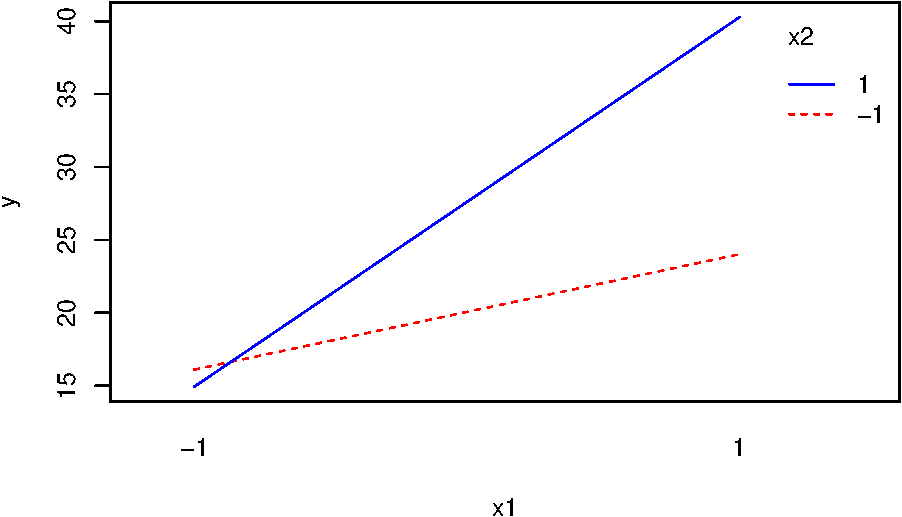
\includegraphics{hw9_files/figure-latex/unnamed-chunk-5-1.pdf}

Interaction plot of the additive model:

\begin{Shaded}
\begin{Highlighting}[]
\NormalTok{add.mod }\OtherTok{=} \FunctionTok{lm}\NormalTok{(y}\SpecialCharTok{\textasciitilde{}}\NormalTok{x1}\SpecialCharTok{+}\NormalTok{x2,}\AttributeTok{data=}\NormalTok{data)}
\NormalTok{add.pred }\OtherTok{=} \FunctionTok{predict}\NormalTok{(add.mod)}
\FunctionTok{interaction.plot}\NormalTok{(data}\SpecialCharTok{$}\NormalTok{x1,data}\SpecialCharTok{$}\NormalTok{x2,add.pred,}
                 \AttributeTok{col=}\FunctionTok{c}\NormalTok{(}\StringTok{"red"}\NormalTok{,}\StringTok{"blue"}\NormalTok{),}
                 \AttributeTok{trace.label=}\StringTok{"x2"}\NormalTok{,}
                 \AttributeTok{xlab=}\StringTok{"x1"}\NormalTok{,}
                 \AttributeTok{ylab=}\StringTok{"y"}\NormalTok{)}
\end{Highlighting}
\end{Shaded}

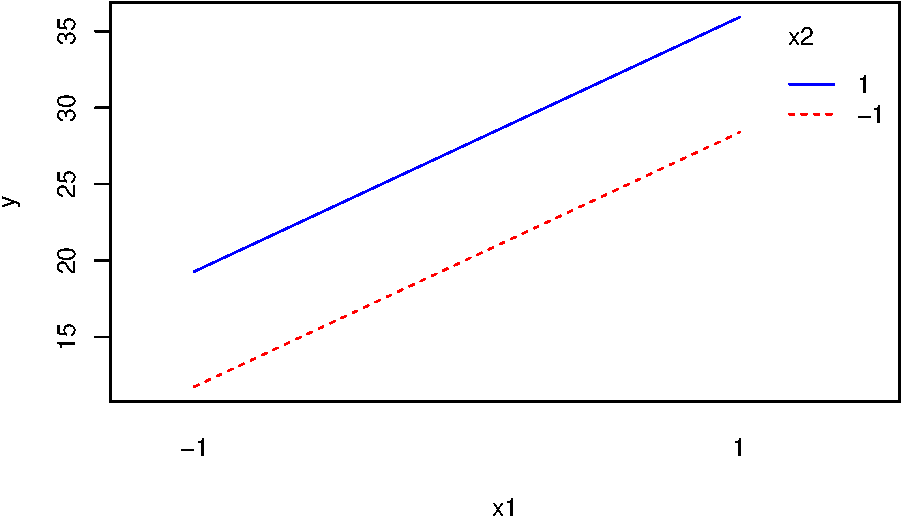
\includegraphics{hw9_files/figure-latex/unnamed-chunk-6-1.pdf}

\hypertarget{part-e}{%
\subsection{Part (e)}\label{part-e}}

\begin{quote}
Test for an interaction effect. (Compute the test statistic and
p-value.) Provide an interpretation, stated in the context of the
problem.
\end{quote}

\begin{Shaded}
\begin{Highlighting}[]
\FunctionTok{anova}\NormalTok{(add.mod,x.mod)}
\end{Highlighting}
\end{Shaded}

\begin{longtable}[]{@{}rrrrrr@{}}
\toprule
Res.Df & RSS & Df & Sum of Sq & F & Pr(\textgreater F) \\
\midrule
\endhead
13 & 375.3531 & NA & NA & NA & NA \\
12 & 71.7225 & 1 & 303.6306 & 50.8009 & 1.2e-05 \\
\bottomrule
\end{longtable}

\(F^* \approx 50\) is quite large (\(p = .000\)). We find the data to be
incompatible with the additive model.

\hypertarget{problem-2}{%
\section{Problem 2}\label{problem-2}}

\begin{quote}
A sample of healthy females is selected to investigate the relationship
between age (\(x\)) and the level of a steroid (\(y\)). Refer to the
data from Exercise 8.6.
\end{quote}

\hypertarget{part-a-1}{%
\subsection{Part (a)}\label{part-a-1}}

\begin{quote}
Fit a quadratic model using coded variables. Compute \(R^2\) for the
quadratic model.
\end{quote}

\begin{Shaded}
\begin{Highlighting}[]
\NormalTok{data }\OtherTok{=} \FunctionTok{read.table}\NormalTok{(}\StringTok{\textquotesingle{}CH08PR06.txt\textquotesingle{}}\NormalTok{)}
\FunctionTok{names}\NormalTok{(data) }\OtherTok{=} \FunctionTok{c}\NormalTok{(}\StringTok{\textquotesingle{}y\textquotesingle{}}\NormalTok{,}\StringTok{\textquotesingle{}x\textquotesingle{}}\NormalTok{)}
\FunctionTok{head}\NormalTok{(data)}
\end{Highlighting}
\end{Shaded}

\begin{longtable}[]{@{}rr@{}}
\toprule
y & x \\
\midrule
\endhead
27.1 & 23 \\
22.1 & 19 \\
21.9 & 25 \\
10.7 & 12 \\
1.4 & 8 \\
18.8 & 12 \\
\bottomrule
\end{longtable}

\begin{Shaded}
\begin{Highlighting}[]
\CommentTok{\# poly uses coded variables (orthogonal)}
\CommentTok{\#     =\textgreater{} z1 = a1 + b1 x}
\CommentTok{\#        z2 = a2 + b2 x + c2 x\^{}2}
\NormalTok{quad.mod }\OtherTok{=} \FunctionTok{lm}\NormalTok{(y }\SpecialCharTok{\textasciitilde{}} \FunctionTok{poly}\NormalTok{(x,}\DecValTok{2}\NormalTok{),}\AttributeTok{data=}\NormalTok{data)}
\FunctionTok{coef}\NormalTok{(quad.mod)}
\end{Highlighting}
\end{Shaded}

\begin{verbatim}
## (Intercept) poly(x, 2)1 poly(x, 2)2 
##    17.64444    28.16524   -15.90551
\end{verbatim}

\begin{Shaded}
\begin{Highlighting}[]
\NormalTok{r2 }\OtherTok{=} \FunctionTok{summary}\NormalTok{(quad.mod)}\SpecialCharTok{$}\NormalTok{r.squared}
\NormalTok{r2}
\end{Highlighting}
\end{Shaded}

\begin{verbatim}
## [1] 0.8143372
\end{verbatim}

The estimate for the quadratic regression model is \[
  E(Y|x) = 17.644 + 28.165 x - 15.906 x^2,
\] for which \[
  R^2 = 0.8143372.
\]

\hypertarget{part-b-1}{%
\subsection{Part (b)}\label{part-b-1}}

\begin{quote}
Fit a cubic model using coded variables. Compute \(R^2\) for the cubic
model.
\end{quote}

\begin{Shaded}
\begin{Highlighting}[]
\NormalTok{cubic.mod }\OtherTok{=} \FunctionTok{lm}\NormalTok{(y }\SpecialCharTok{\textasciitilde{}} \FunctionTok{poly}\NormalTok{(x,}\DecValTok{3}\NormalTok{),}\AttributeTok{data=}\NormalTok{data)}
\FunctionTok{coef}\NormalTok{(cubic.mod)}
\end{Highlighting}
\end{Shaded}

\begin{verbatim}
## (Intercept) poly(x, 3)1 poly(x, 3)2 poly(x, 3)3 
##   17.644444   28.165236  -15.905513    4.086111
\end{verbatim}

\begin{Shaded}
\begin{Highlighting}[]
\NormalTok{r2 }\OtherTok{=} \FunctionTok{summary}\NormalTok{(cubic.mod)}\SpecialCharTok{$}\NormalTok{r.squared}
\end{Highlighting}
\end{Shaded}

The estimate for the cubic regression model is \[
  E(Y|x) = 17.644 + 28.165 x - 15.906 x^2 + 4.086 x^3,
\] which, given the orthogonal design, has the same coefficients as
previously for the lower-order terms.

As expected, \(R^2\) has increased, \[
  R^2 = 0.8273324,
\] but only slightly.

\hypertarget{part-c-1}{%
\subsection{Part (c)}\label{part-c-1}}

\begin{quote}
Create a scatterplot of the data, comparing the fitted values from the
quadratic model with the fitted values from the cubic model. Extrapolate
the predictions \(10\) years beyond the largest age in the data set.
\end{quote}

\begin{Shaded}
\begin{Highlighting}[]
\NormalTok{newdat }\OtherTok{=} \FunctionTok{data.frame}\NormalTok{(}\AttributeTok{x=}\FunctionTok{seq}\NormalTok{(}\FunctionTok{min}\NormalTok{(data}\SpecialCharTok{$}\NormalTok{x),}\FunctionTok{max}\NormalTok{(data}\SpecialCharTok{$}\NormalTok{x)}\SpecialCharTok{+}\DecValTok{10}\NormalTok{,}\AttributeTok{length.out=}\DecValTok{100}\NormalTok{))}
\NormalTok{newdat}\SpecialCharTok{$}\NormalTok{cubic.pred }\OtherTok{=} \FunctionTok{predict}\NormalTok{(cubic.mod, }\AttributeTok{newdata =}\NormalTok{ newdat)}
\NormalTok{newdat}\SpecialCharTok{$}\NormalTok{quad.pred }\OtherTok{=} \FunctionTok{predict}\NormalTok{(quad.mod, }\AttributeTok{newdata =}\NormalTok{ newdat)}
                          
\FunctionTok{plot}\NormalTok{(data}\SpecialCharTok{$}\NormalTok{x,data}\SpecialCharTok{$}\NormalTok{y,}
     \AttributeTok{xlim=}\FunctionTok{c}\NormalTok{(}\FunctionTok{min}\NormalTok{(data}\SpecialCharTok{$}\NormalTok{x),}\FunctionTok{max}\NormalTok{(data}\SpecialCharTok{$}\NormalTok{x)}\SpecialCharTok{+}\DecValTok{10}\NormalTok{),}
     \AttributeTok{ylim=}\FunctionTok{c}\NormalTok{(}\DecValTok{0}\NormalTok{,}\DecValTok{40}\NormalTok{),}
     \AttributeTok{xlab=}\StringTok{"x"}\NormalTok{,}
     \AttributeTok{ylab=}\StringTok{"y"}\NormalTok{)}
\FunctionTok{legend}\NormalTok{(}\DecValTok{16}\NormalTok{, }\DecValTok{8}\NormalTok{, }\AttributeTok{legend=}\FunctionTok{c}\NormalTok{(}\StringTok{"cubic"}\NormalTok{,}\StringTok{"quadratic"}\NormalTok{),}
       \AttributeTok{col=}\FunctionTok{c}\NormalTok{(}\StringTok{"red"}\NormalTok{,}\StringTok{"green"}\NormalTok{), }\AttributeTok{lty=}\DecValTok{1}\SpecialCharTok{:}\DecValTok{1}\NormalTok{, }\AttributeTok{cex=}\FloatTok{0.8}\NormalTok{)}
\FunctionTok{points}\NormalTok{(newdat}\SpecialCharTok{$}\NormalTok{x,newdat}\SpecialCharTok{$}\NormalTok{cubic.pred,}\AttributeTok{type=}\StringTok{"l"}\NormalTok{,}\AttributeTok{col=}\StringTok{"red"}\NormalTok{)}
\FunctionTok{points}\NormalTok{(newdat}\SpecialCharTok{$}\NormalTok{x,newdat}\SpecialCharTok{$}\NormalTok{quad.pred,}\AttributeTok{type=}\StringTok{"l"}\NormalTok{,}\AttributeTok{col=}\StringTok{"green"}\NormalTok{)}
\end{Highlighting}
\end{Shaded}

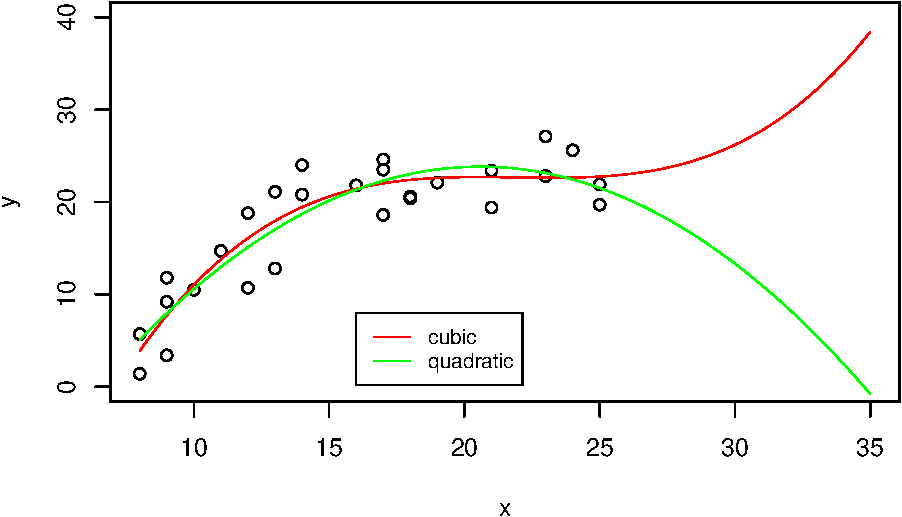
\includegraphics{hw9_files/figure-latex/unnamed-chunk-10-1.pdf}

Informally, unless we have prior information (e.g., scientific insight),
the simpler (quadradic) model seems like a more likely fit to the
underlying data generating process.

\end{document}
